\clearpage
\onecolumn
 
\setcounter{page}{1}
\maketitlesupplementary
 
\section{Ergänzende Abbildungen}
\label{sec:supp_figures}
 
% ----------------------------------------------------------
% Seite 1: beide Tabellen in natürlicher Größe
% ----------------------------------------------------------
 
\begin{table}[H]
	\centering
	\caption{Vergleich der Trainingsläufe: Testgenauigkeit, Validierungsgenauigkeit und Validierungsverlust nach 15 Epochen sowie die benötigte Trainingszeit. Als Baseline dient das ohne Teacher trainierte Student-Netz. Das beste Ergebnis ist fett hervorgehoben.}
	\label{tab:distillation_ergebnisse}
	\begin{tabular}{llrrrr}
		\toprule
		$\alpha$ & $T$ & Acc\textsubscript{Test} [\%] & Acc\textsubscript{Val} [\%] & Loss\textsubscript{Val} & Zeit [min] \\
		\midrule
		\multicolumn{2}{l}{Baseline (ohne Teacher)} & 73{,}16 & 75{,}44 & 0{,}899 & 2{,}44 \\
		\midrule
		0{,}1 & 2{,}0 & 71{,}40          & 72{,}28          & 1{,}492          & 6{,}57 \\
		0{,}1 & 4{,}0 & \textbf{82{,}11} & \textbf{84{,}04} & \textbf{0{,}671} & 6{,}65 \\
		0{,}1 & 6{,}0 & 77{,}37          & 79{,}65          & 1{,}058          & 6{,}66 \\
		0{,}2 & 2{,}0 & 78{,}95          & 79{,}12          & 0{,}870          & 6{,}70 \\
		0{,}2 & 4{,}0 & 76{,}49          & 75{,}96          & 1{,}370          & 6{,}75 \\
		0{,}2 & 6{,}0 & 80{,}18          & 77{,}72          & 1{,}038          & 6{,}75 \\
		0{,}3 & 2{,}0 & 72{,}98          & 75{,}61          & 1{,}093          & 7{,}68 \\
		0{,}3 & 4{,}0 & 76{,}84          & 79{,}47          & 0{,}971          & 6{,}71 \\
		0{,}3 & 6{,}0 & 74{,}39          & 74{,}91          & 1{,}301          & 6{,}84 \\
		\bottomrule
	\end{tabular}
\end{table}
 
\vspace{1.5em}
 
\begin{table}[H]
	\centering
	\caption{Übersicht der getesteten Netzarchitekturen. Conv = Anzahl Convolution-Layern, Pool = Anzahl Max-Pooling-Schichten, FC = Anzahl vollständig verbundener Schichten (inkl. Ausgabeschicht), BN = Batch-Normalisierung, DO = Dropout ($p = 0{,}5$).}
	\label{tab:architektur_uebersicht}
	\begin{tabular}{llccccc}
		\toprule
		\textbf{Phase} & \textbf{Netzwerk}                              & \textbf{Conv} & \textbf{Pool} & \textbf{FC} & \textbf{BN} & \textbf{DO} \\
		\midrule
		1              & Base\_Net                                      & 5             & 2 + GAP       & 3           & --          & --          \\
		\midrule
		2              & Conv\_Net                                      & 8             & 2             & 3           & --          & --          \\
		2              & Dense\_Net                                     & 5             & 2             & 7           & --          & --          \\
		2              & Pooling\_Net                                   & 5             & 4             & 3           & --          & --          \\
		2              & Dropout\_Net                                   & 5             & 2             & 3           & --          & \checkmark  \\
		2              & BatchNorm\_Net                                 & 5             & 2             & 3           & \checkmark  & --          \\
		\midrule
		3              & BatchNorm\_Dense\_Pool\_Net                    & 5             & 3             & 4           & \checkmark  & --          \\
		3              & BatchNorm\_Dense\_Pool\_Conv\_Net              & 6             & 3             & 4           & \checkmark  & --          \\
		3              & BatchNorm\_Dense\_Pool\_Conv\_Dropout\_Net     & 6             & 3             & 4           & \checkmark  & \checkmark  \\
		3              & BatchNorm\_Dense\_Pool\_Conv\_Dropout\_V2\_Net & 6             & 3             & 4           & \checkmark  & \checkmark  \\
		\bottomrule
	\end{tabular}
\end{table}
 
\clearpage
\onecolumn
% ----------------------------------------------------------
% Seite 2: Loss-Verläufe
% ----------------------------------------------------------
 
\begin{figure}[H]
	\centering
	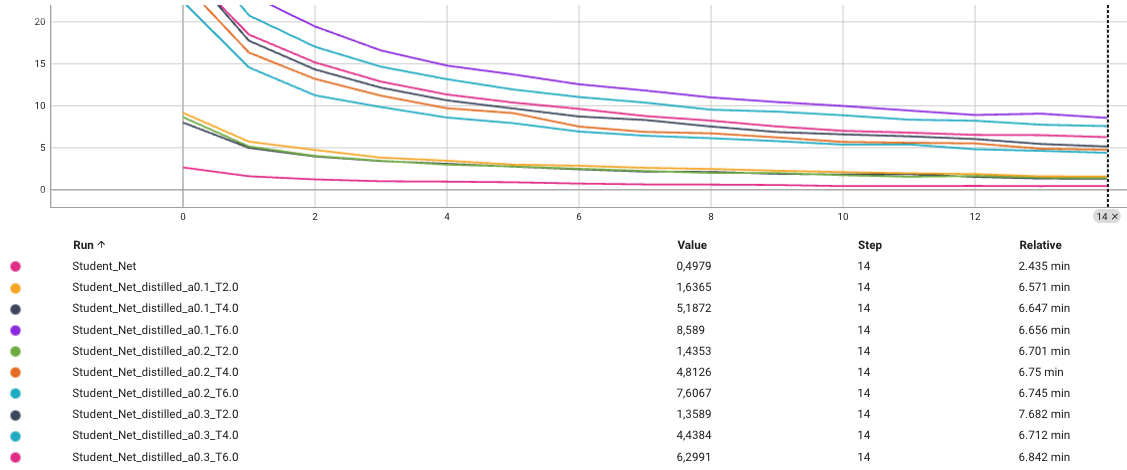
\includegraphics[width=\linewidth, height=0.85\textheight, keepaspectratio]{figures/loss.png}
	\caption{Verlauf des Trainingsverlusts über 15 Epochen für alle Konfigurationen.}
	\label{fig:train_loss}
\end{figure}

\begin{figure}[H]
	\centering
	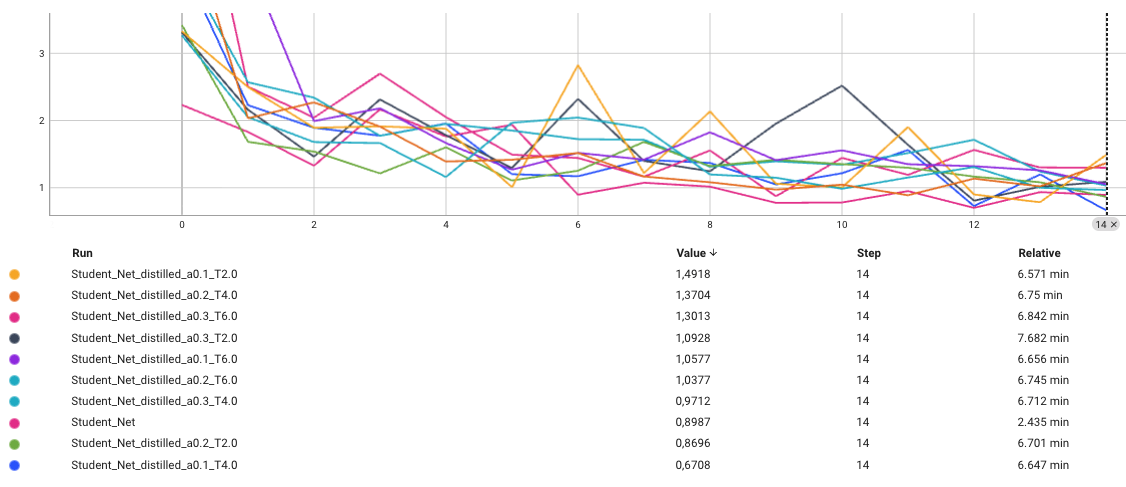
\includegraphics[width=\linewidth, height=0.85\textheight, keepaspectratio]{figures/val_loss.png}
	\caption{Verlauf des Validierungsverlusts über 15 Epochen für alle Konfigurationen.}
	\label{fig:val_loss}
\end{figure}
 
\clearpage
\onecolumn

% ----------------------------------------------------------
% Seite 3 und 4: je eine Konfusionsmatrix pro Seite
% ----------------------------------------------------------
 
\begin{figure}[H]
	\centering
	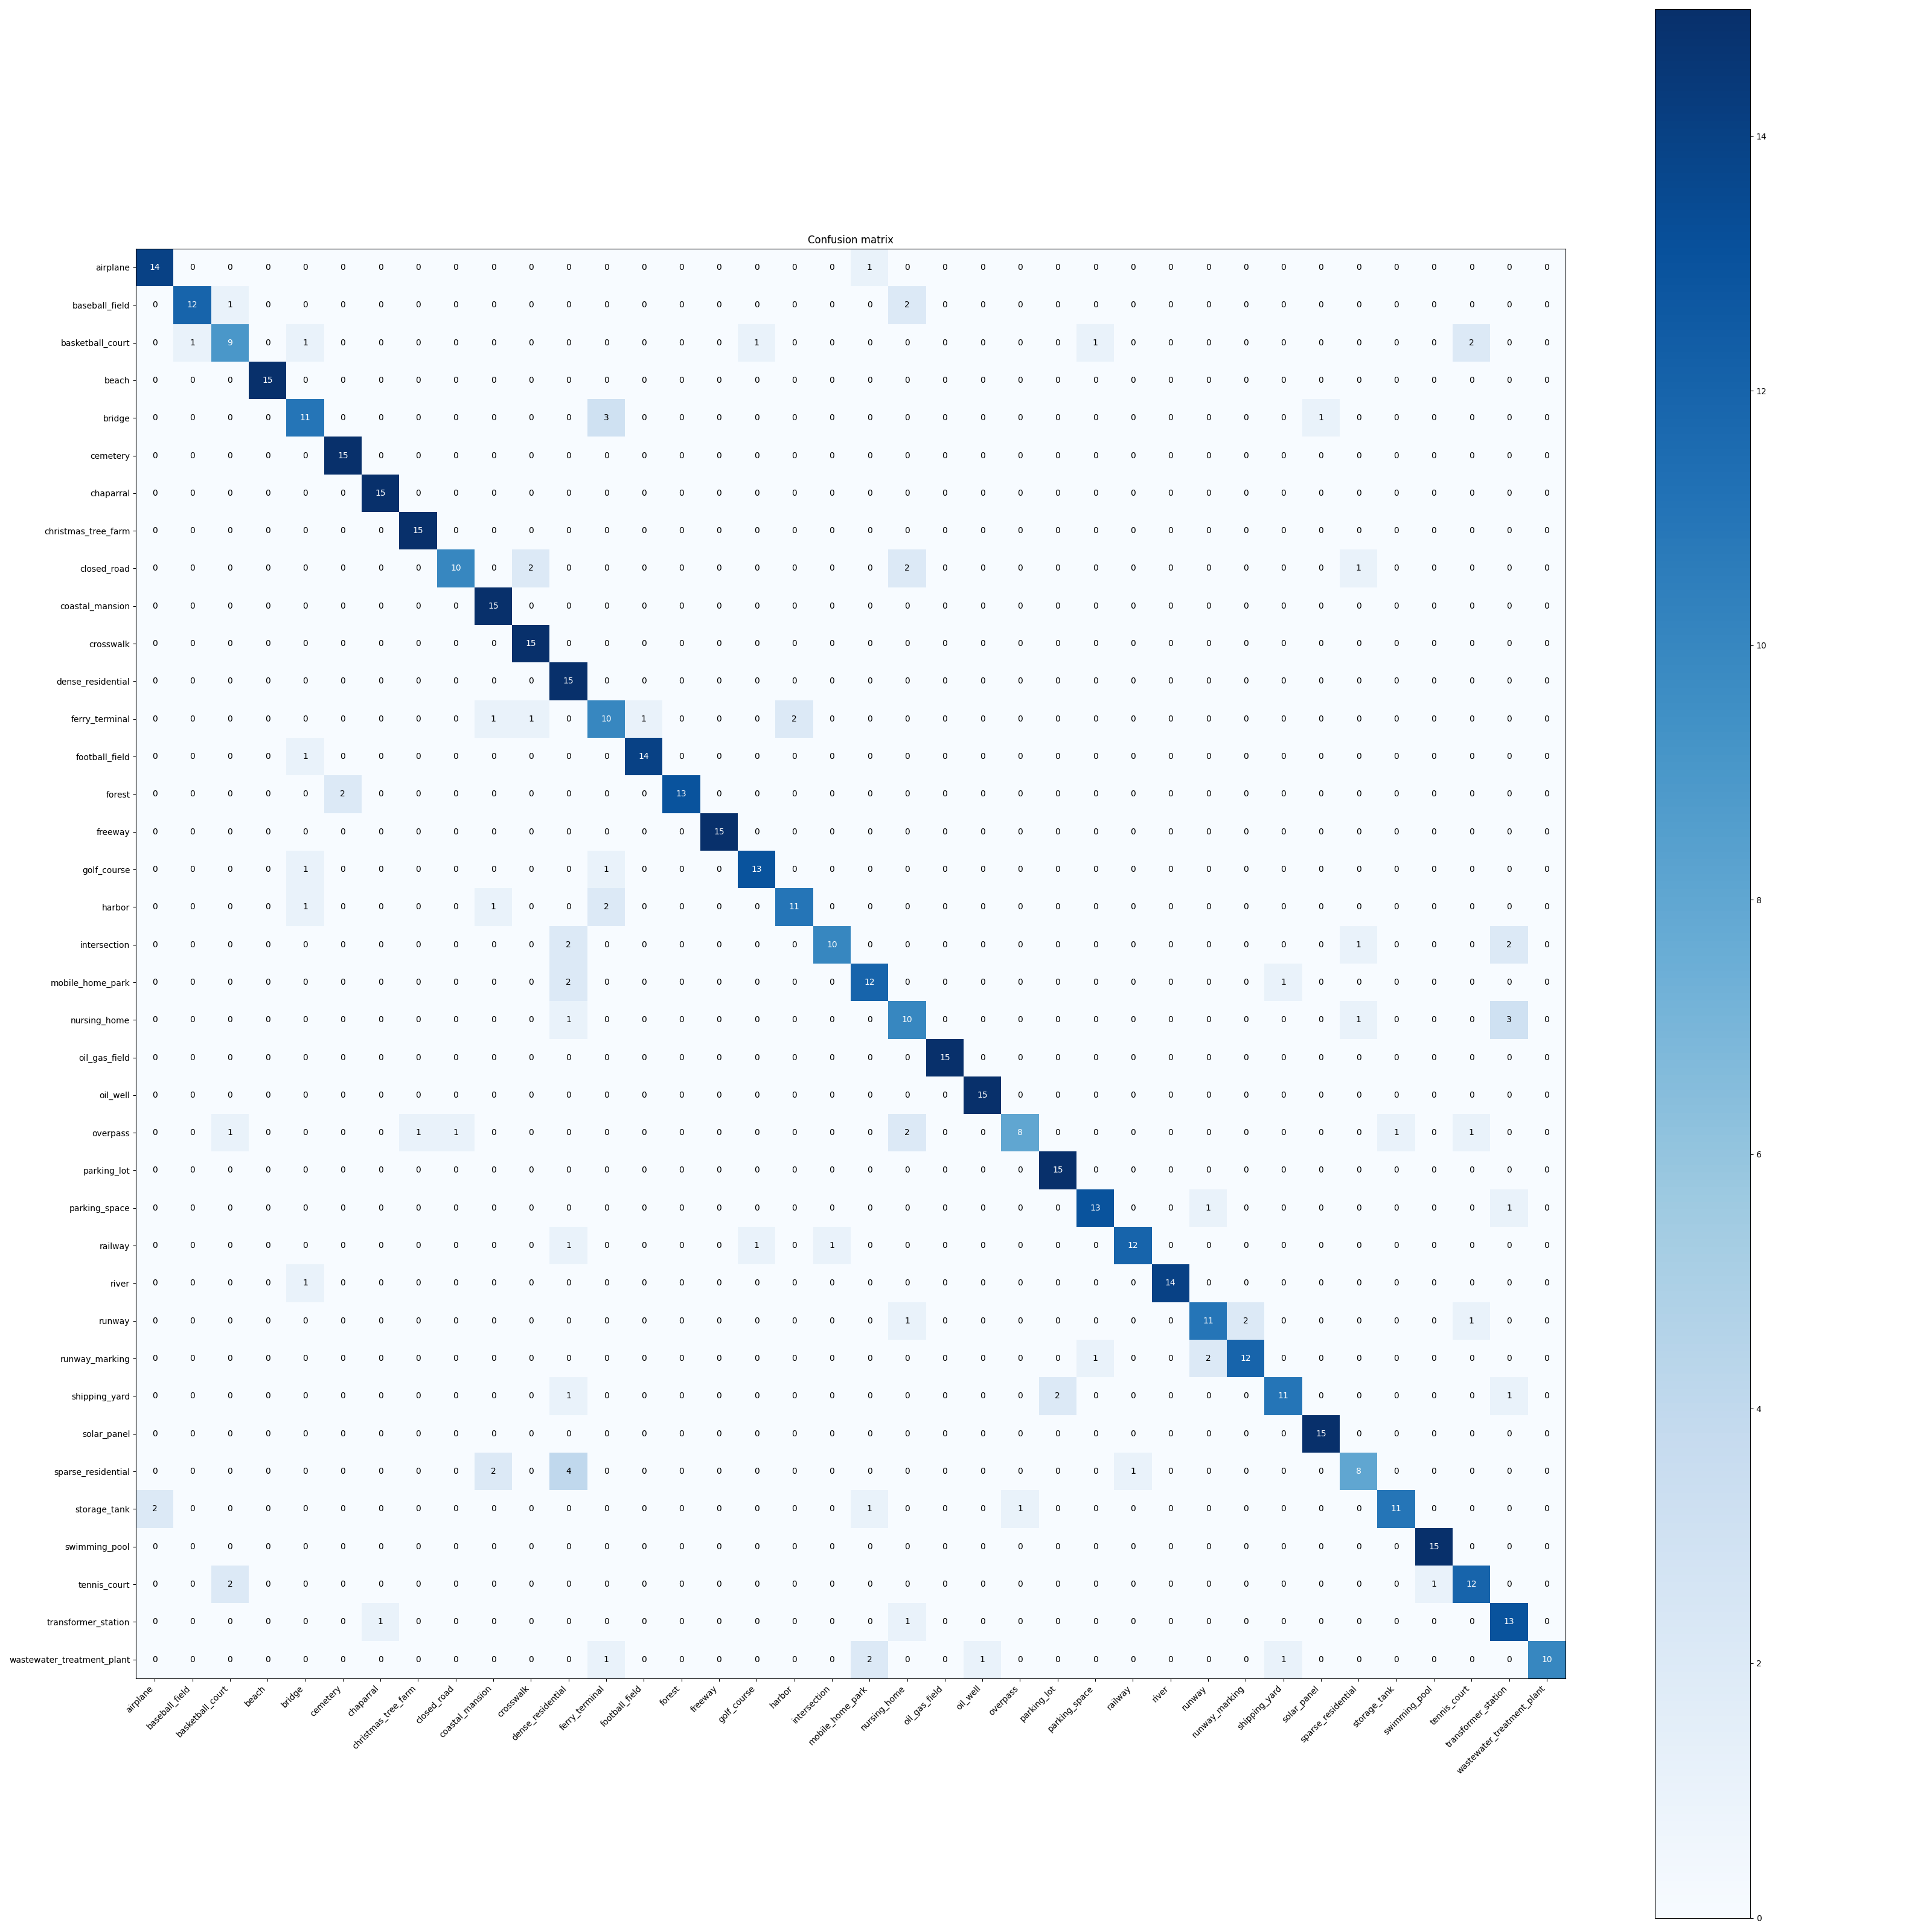
\includegraphics[width=\linewidth, height=0.88\textheight, keepaspectratio]{figures/cm_distilled_a01_T4.png}
	\caption{Konfusionsmatrix des besten destillierten Modells ($\alpha = 0{,}1$, $T = 4{,}0$) auf dem Testdatensatz.}
	\label{fig:cm_distilled}
\end{figure}
 
\clearpage
 
\begin{figure}[H]
	\centering
	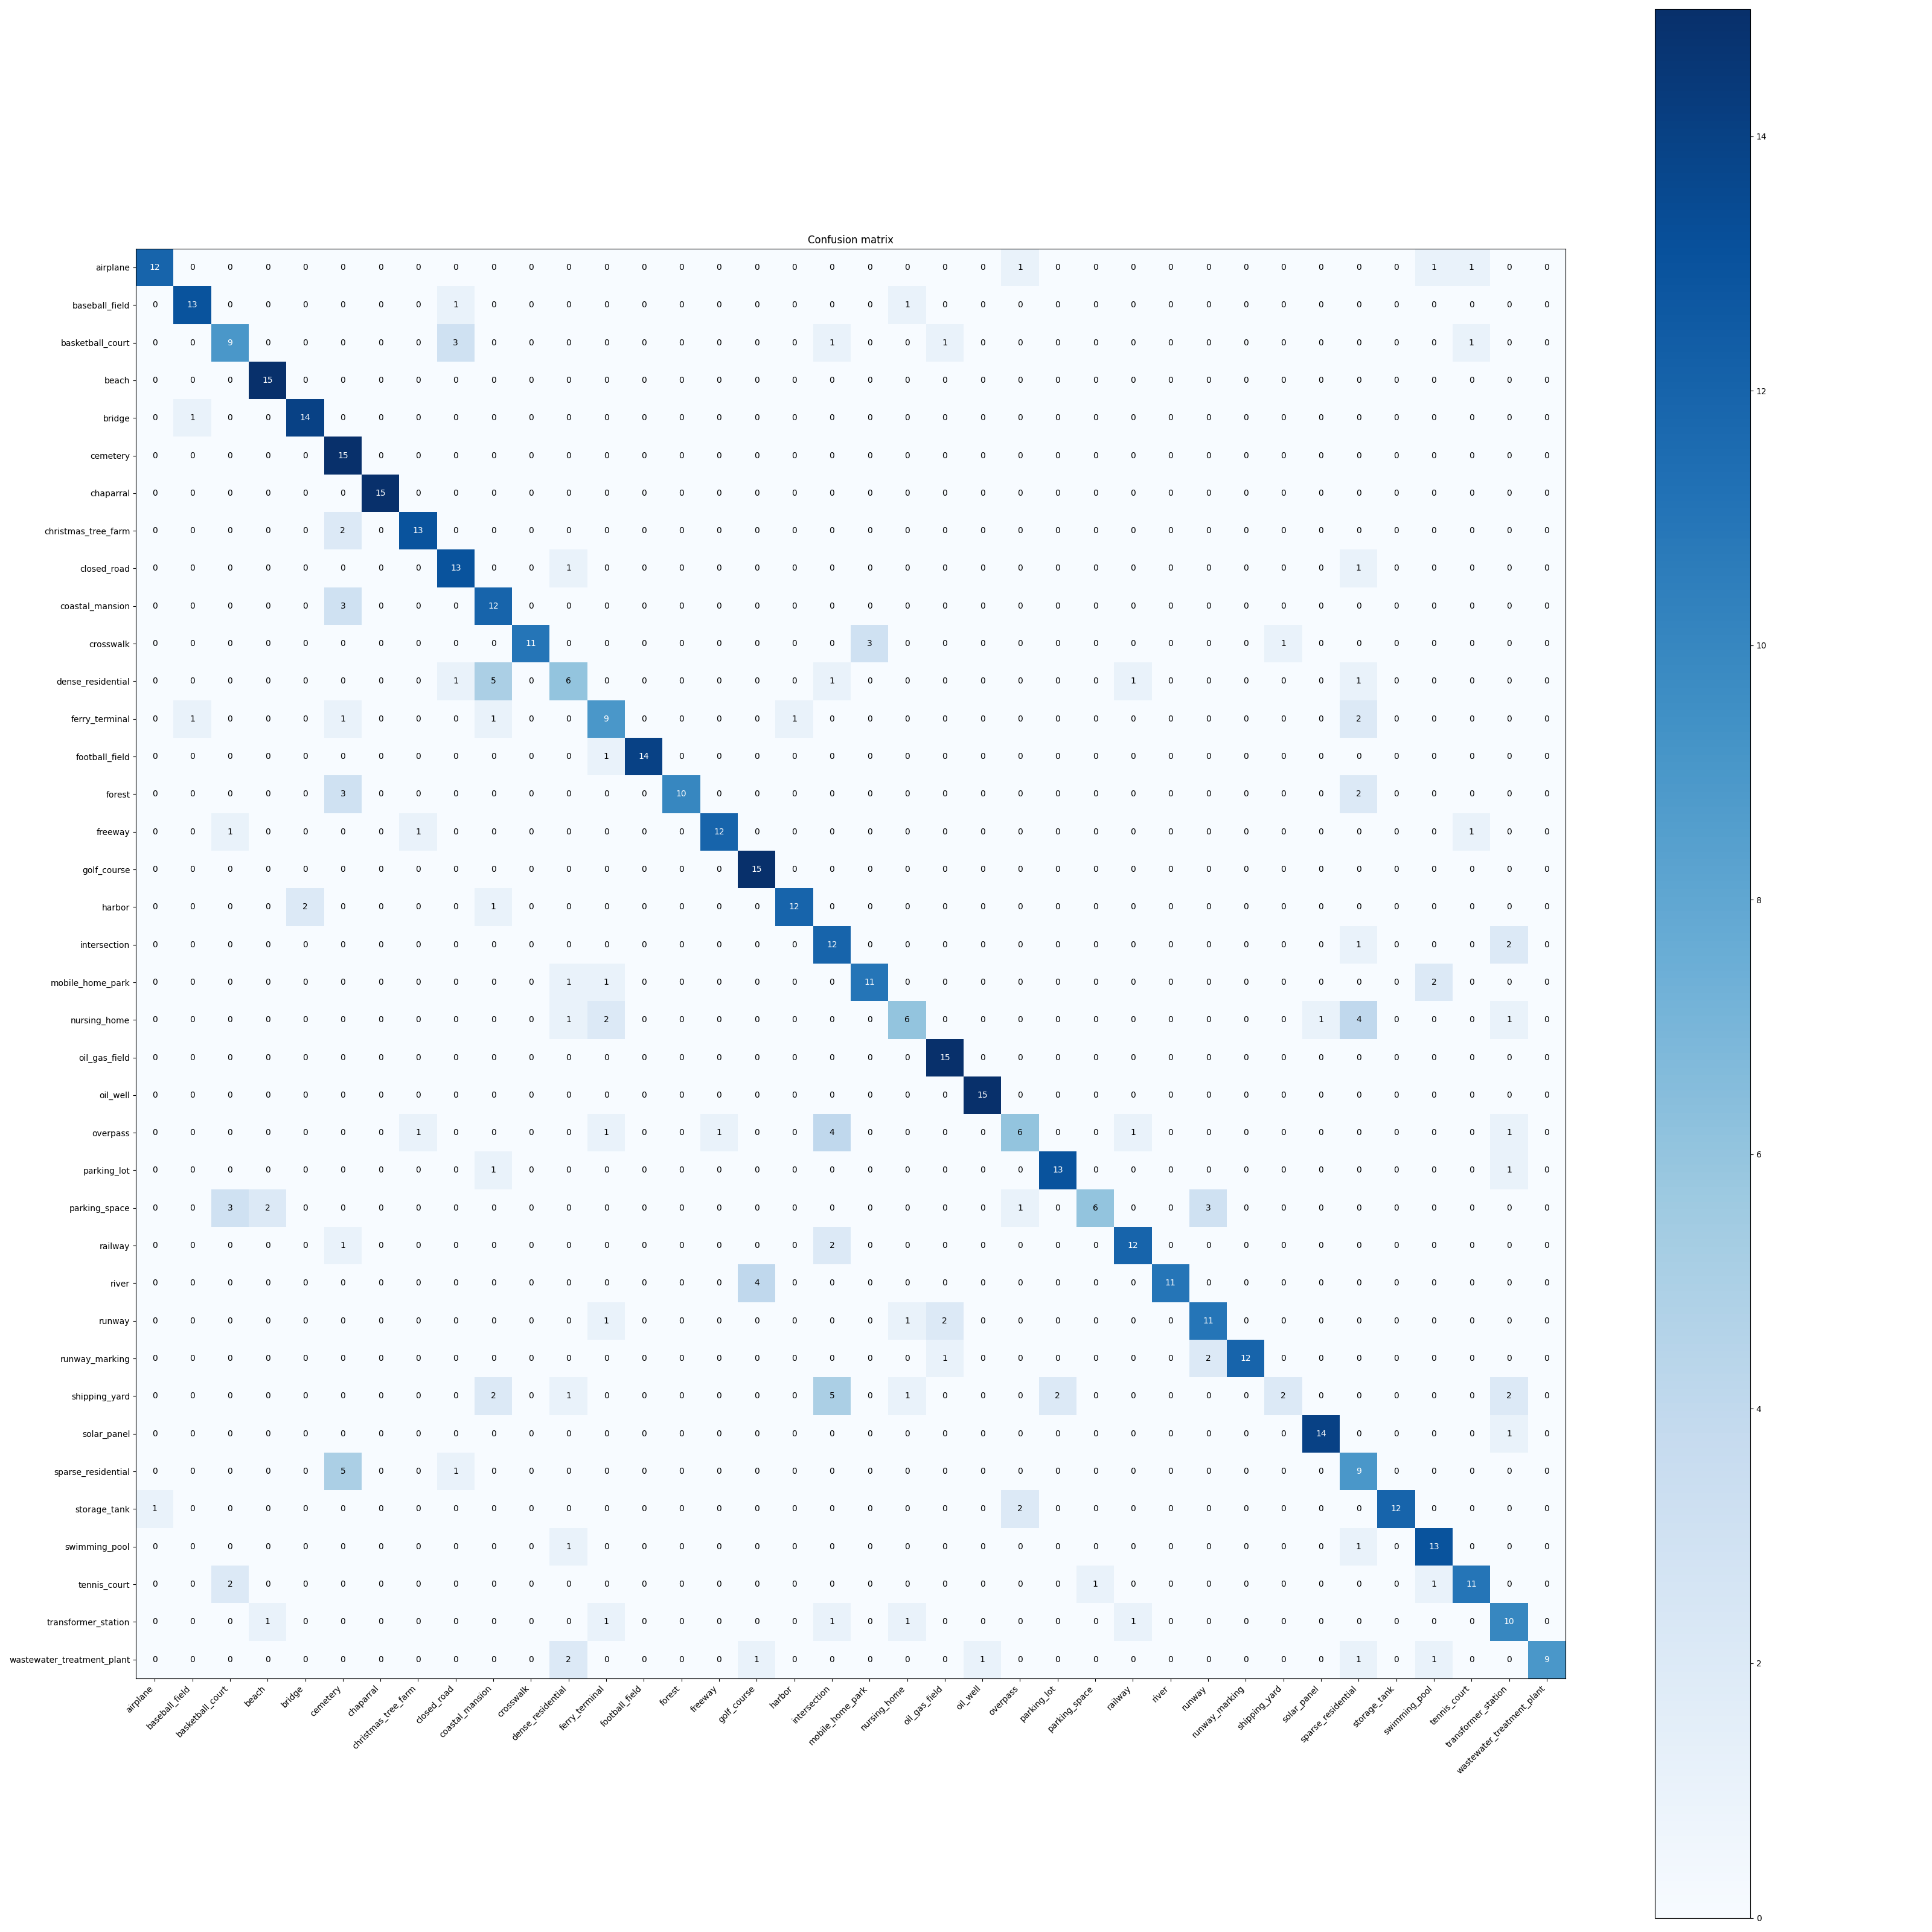
\includegraphics[width=\linewidth, height=0.88\textheight, keepaspectratio]{figures/cm_baseline.png}
	\caption{Konfusionsmatrix des ohne Teacher trainierten Student-Netzes (Baseline) auf dem Testdatensatz.}
	\label{fig:cm_baseline}
\end{figure}